\chapter{ABOUT WOFOST 6.0}

The processes which characterize crop growth, have to be ordered in a rational way to
simulate crop growth. This manual describes these processes as they are imple\-ment\-ed in
WOFOST 6.0. The subroutines are presented in relation to the described process\-es. 

This chapter provides some basic information on the development of WOFOST (\S 2.1),
the applications of WOFOST (\S 2.2) and on the function\-ality of WOFOST (\S 2.3). Chapter
3 provides information on the structure of the Euler integra\-tion which is used to integrate
the variables over time. Chapter 4 discusses the calculation and conversion of meteorolog\-ical data like: calculation of potential evapo\-(trans)piration, calculation of day length and
solar elevation. Chapter 5 discusses how the crop growth processes are simulated like:
daily assimilation, mainte\-nance respiration, growth respira\-tion, parti\-tioning of assimilates,
senes\-cence and death. Chapter 6 discusses the soil water balance calcula\-tions. These
calculations are used to keep track of the water in the soil. The soil moisture content can
be calculated from this.

It should be mentioned that two versions of WOFOST 6.0 exist. One is the version
currently implemented in the CGMS system of the Joint Research Centre of the EC, at
Ispra, Italy. The other version is a more general version. In Appendix 5 the differences
between these two versions will be briefly explained. However, the processes which
describe the crop growth do not differ in both versions. They will be explained in the
following text.

\section{\index{WOFOST}Development of WOFOST}

WOFOST originated in the framework of an interdisciplinary study on the potential world
food production by the Centre for World Food Studies (CWFS) in coopera\-tion with the
Wageningen Agricultu\-ral Univer\-sity, Depart\-ment of Theoretical Production Ecology
(WAU-TPE) and the DLO-Centre for Agrobiolo\-gi\-cal Re\-search (CABO-DLO, currently
AB-DLO), Wagenin\-gen, the Nether\-lands. After cessa\-tion of the CWFS in 1988, the 
deve\-lopment of the model has been carried out at the DLO-Winand Staring Centre (SC-DLO)
in cooperation with AB-DLO and WAU-TPE.

WOFOST is a member of the family of models developed in Wageningen by the school
of C.T. de Wit. Related models are the successive SUCROS models (Simple and
Universal Crop Simu\-lator) (Spitters {\it et al}., 1989; Van Laar {\it et al}., 1992), Arid Crop (Van
Keulen, 1975; Van Keulen {\it et al.}, 1981), Spring wheat (Van Keulen and Seligman, 1987;
Stol et al., 1993), MACROS (Penning de Vries et al., 1989) and ORYZA1 (Kropff et al.,
1993). The first WOFOST model has been documented by Wolf {\it et al}. (1986).

All these Wageningen models follow the hierarchical distinc\-tion between potential and
limited production, and share similar crop growth submodels, with light interception and
CO$_{{\rm 2}}$ assimilation as growth driving processes, and crop phenological development as
growth controlling process. How\-ever, the submodels describing the soil water balance and
the crop nutrient uptake vary much in approach and level of detail.

The development of WOFOST has been connected to the need for its application in
several studies. Although most of these studies did not have the specific purpose to
develop the model as such, efforts were made to maintain parts of the software developed
as options in the subsequent model versions.

WOFOST was originally developed as a crop growth simulation model for the assessment
of the yield potential of various annual crops in tropi\-cal countries (Van Keulen and Wolf,
1986; Van Diepen {\it et al.}, 1988; Van Keulen and Van Diepen, 1990). At first it was tried
to keep the need for input data as low as possible, by using average input values.
However, it soon became clear that the variability of the environmental condi\-tions
determining crop growth, both in space and time, had to be taken into account. The use
of long term mean monthly weather data, mean sowing dates, and averaged soil data as
model input may lead to a false impression of the agroecologic potential of a region.
This implies that original rather than averaged data must be used as model input and that,
if needed, averaging can be done only {\it after} the simula\-tion. In other words: calculate first
and average later (De Wit and Van Keulen, 1987; Nonhebel, 1994).

\section{\index{WOFOST}Applications of WOFOST  }

Over the last ten years, the successive WOFOST versions and their derivates have been
used in many studies. WOFOST has been applied as a tool for the analysis of yield risk
and inter-annual yield variability, of yield variability over soil types, or over a range of
agrohydrological conditions, of differences between cultivars, of relative importance of
growth determining factors, of sowing strategies, effects of climate change and critical
periods for use of agricultural machinery. The model has also been used for predictive
pur\-poses, in quantitative land evaluation, such as regional assessments of crop yield
potential in the form of maximum yield levels, estimation of maximum benefits from
irrigation or from fertilizer use, detection of adverse growing condi\-tions by 
simulation-monitoring the agricultural season, and regional yield forecasts. Some WOFOST 
workers have extended the growth model to forest and grass, and have replaced the soil water
module by more detailed submodels.

Unfortunately, a complete overview of applications of WOFOST is not available, since
there has never been a formal network or newsletter for exchange of experiences and
(validat\-ed) data sets. This has severely hampered feedback to the model devel\-opers. Here,
we mention the major application studies that influenced its development, and a few
examples of other WOFOST applications and extensions.

The first major regional study on the basis of WOFOST (version 3.1) dealt with potential
food production increases from fertilizer aid in three African countries, and was carried
out by the CWFS at the request of the FAO. The study indicated that yield of food crops
in Burkina Faso, Ghana and Kenya could be increased substantially with increased
fertilizer use without requiring additional irrigation (CWFS, 1985).

Within the framework of the Monitoring Agro-ecological resources with Remote sensing
and Simulation (MARS) project, WOFOST (version 4.1) has been proposed as a yield
estimating tool in an early warning system for food security in Zambia. This system
would consist of a GIS (Geographic Information System) and a crop model, and would be
fed with data from meteorological satellites (Berkhout {\it et al}., 1988). For that purpose the
WOFOST model has been calibrated and tested for maize (Huygen, 1990; Wolf {\it et al}.,
1989). WOFOST 4.1 was also applied to evaluate irrigation and water conservation 
strat\-egies in support of rural development in small watersheds in the Peruvian Andes 
(Van der Zel, 1989).

An elaborated calibration and validation study for maize in Kenya was carried out by
R\"{o}tter (1993) on the basis of WOFOST 4.4. Using data from experimental fields he
found that the model predicted grain yields with an accuracy of 15 percent (Root Mean
Square Error) which was considered satisfactory in the light of the quality of the available
data. WOFOST was then applied to re-evaluate former field trials with varying planting
dates and fertilizer treatments and to assess yield risks for specific sites, prior to
interpolation to regions using GIS techniques.

The AGRISK project applied WOFOST for risk studies in Burkina Faso, in order to
analyze farmer's strategies to cope with drought risks in relation to soil type, crop and
cultivar, sowing date, runoff and location of crop fields (Mellaart, 1989). Bakker (1992),
studied the scope for rainfall insurance as a part of ICRISAT's village level studies in
India's semi-arid tropics.

In the NASREC program of ISRIC and UNEP supporting the estab\-lishment of National
Soil Reference Collections and Databases for education, extension and research, in which
11 countries participate WOFOST has been adopted as the reference crop model. To
facilitate the use of the model for detailed land/soil properties studies, ISRIC has
developed a user-friendly shell for WOFOST (version 4.3), providing a link to the
NASREC database applications (Pulles {\it et al}., 1991).

WOFOST (version 5.3) was used for the estimation of the regional production potential of
the major field crops in the European Community, as a function of soil and climate 
condi\-tions (De Koning and van Diepen, 1992; van Lanen {\it et al}., 1992). To that end, 
data sets arange of temperate crops (wheat, maize, oilseed rape, potato, sugar beet) were 
devel\-oped as well as a separate model version for grass. In this study the model was linked
to a GIS to facilitate generation of model input data and to aggregate model output over regions.
The data generated were used to determine input-output coefficients of cropping systems
in the EC (De Koning {\it et al}., 1994). These coefficients were used in GOAL (General
Optimum Allocation of Land use), an Interactive Multiple Goal Linear Program\-ming
Model developed by the Netherlands Scien\-tific Council for Government Policy (1992) to
explore feasible options for rural land use in the EC. One of the conclusions of the study
was that in Europe at least 30 percent of the agricultural land could be taken out of
production without endangering food security or compromising other major politi\-cal
objectives.

In other studies WOFOST has been used to asses the effect of climate change on crop
growth (Van Diepen {\it et al}., 1987; Wolf and Van Diepen, 1991; Wolf, 1993). The model
is particularly suited to quantify the com\-bined effect of changes in CO$_{{\rm 2}}$, tempera\-ture,
rainfall and solar radiation, on crop development, crop growth and crop water use, as all
the relevant processes are simulated separately while taking due account of their interac\-tions.

WOFOST version 6 was developed under the contract study "Models for yield forecast\-ing" 
issued by the Joint Research Centre (JRC) of the European Commission at Ispra,
Italy, in the framework of Action 3 of the Agriculture Project, also called MARS project
(Monitoring Agriculture with Remote Sens\-ing). The objective of this study was to
generate crop growth indicators for the quality of the current agricultural season over the
EC regions as compared to the quality of historic seasons, and to use these indicators for
quantitative yield prediction per region and per country. 

To this end WOFOST has been
incorporated in the Crop Growth Monitoring System (CGMS). In CGMS, that runs on a
SUN-UNIX computer, WOFOST is linked to an ORACLE relational data base and an
ARC/Info GIS (Hooijer and Van der Wal, 1994; Van Diepen, 1992). The stand-alone
version of WOFOST 6.0 has been maintained for learning, demon\-stration, test and
validation purposes, and as a starting point for its application in other studies.

In addition to the mainstream of WOFOST versions several models have been elaborated
on the basis of WOFOST 4.1. A typical example is the SWACROP2 model formed by
linking the WOFOST crop module to the SWATRE soil water and transpiration rate
model (Huygen, 1992). Groot (1987) simulated the nitrogen dynamics in crop and soil.
Poels and Bijker (1993) created the model TROPFOR to simulate growth and water use
of tropical rainforest by adapting WOFOST 4.1. De Ruijter {\it et al}. (1993) reshaped
WOFOST into a model simulating tulip growth.

\section{Functionality  }

Crop growth is often described by an empirical model, consisting of a regression equation
(e.g. a logistic function). Sometimes, environmental variables, such as radiation and
rainfall, are incorporated in the regression. These models can generate accurate yield
predictions, especially when the regression parameters are estimated on the basis of
extensive sets of experimental data. The predictions are restricted to the same environ\-ment 
on which the regression is based. These empirical, descriptive models, however,
give little insight into the causes of the observed variation in yields.  

WOFOST 6.0 is a mechanistic model that explains crop growth on the basis of the 
underlying processes, such as photosynthesis and respiration, and how these processes are
influenced by environmental conditions. The predictive ability of mechanistic models does
not always live up to expectation. It should be realized, however, that each parame\-ter
estimate and process formulation has its own inaccura\-cy, and that these errors accumulate
in the prediction of final yield.

The WOFOST model explains crop growth on the basis of the underly\-ing processes, such
as photosynthesis and respira\-tion, and how these processes are influenced by environ\-mental 
conditions. Dry matter accumulation of a crop can thus be calculated as a function
of meteorological parameters such as irradiation, temperature, windspeed, etc. and crop
characteristics. The meteorological data are often measured on a daily basis. This is the
reason why the time step, $\Delta$t (or delt), for simulation is set to one day, which on its turn,
means that crop growth is simulated on a daily basis. Figure 2.1 illustrates how the main
processes are organized in the WOFOST model.

\begin{figure}[htbp]
%Fig. 2.1
\centering
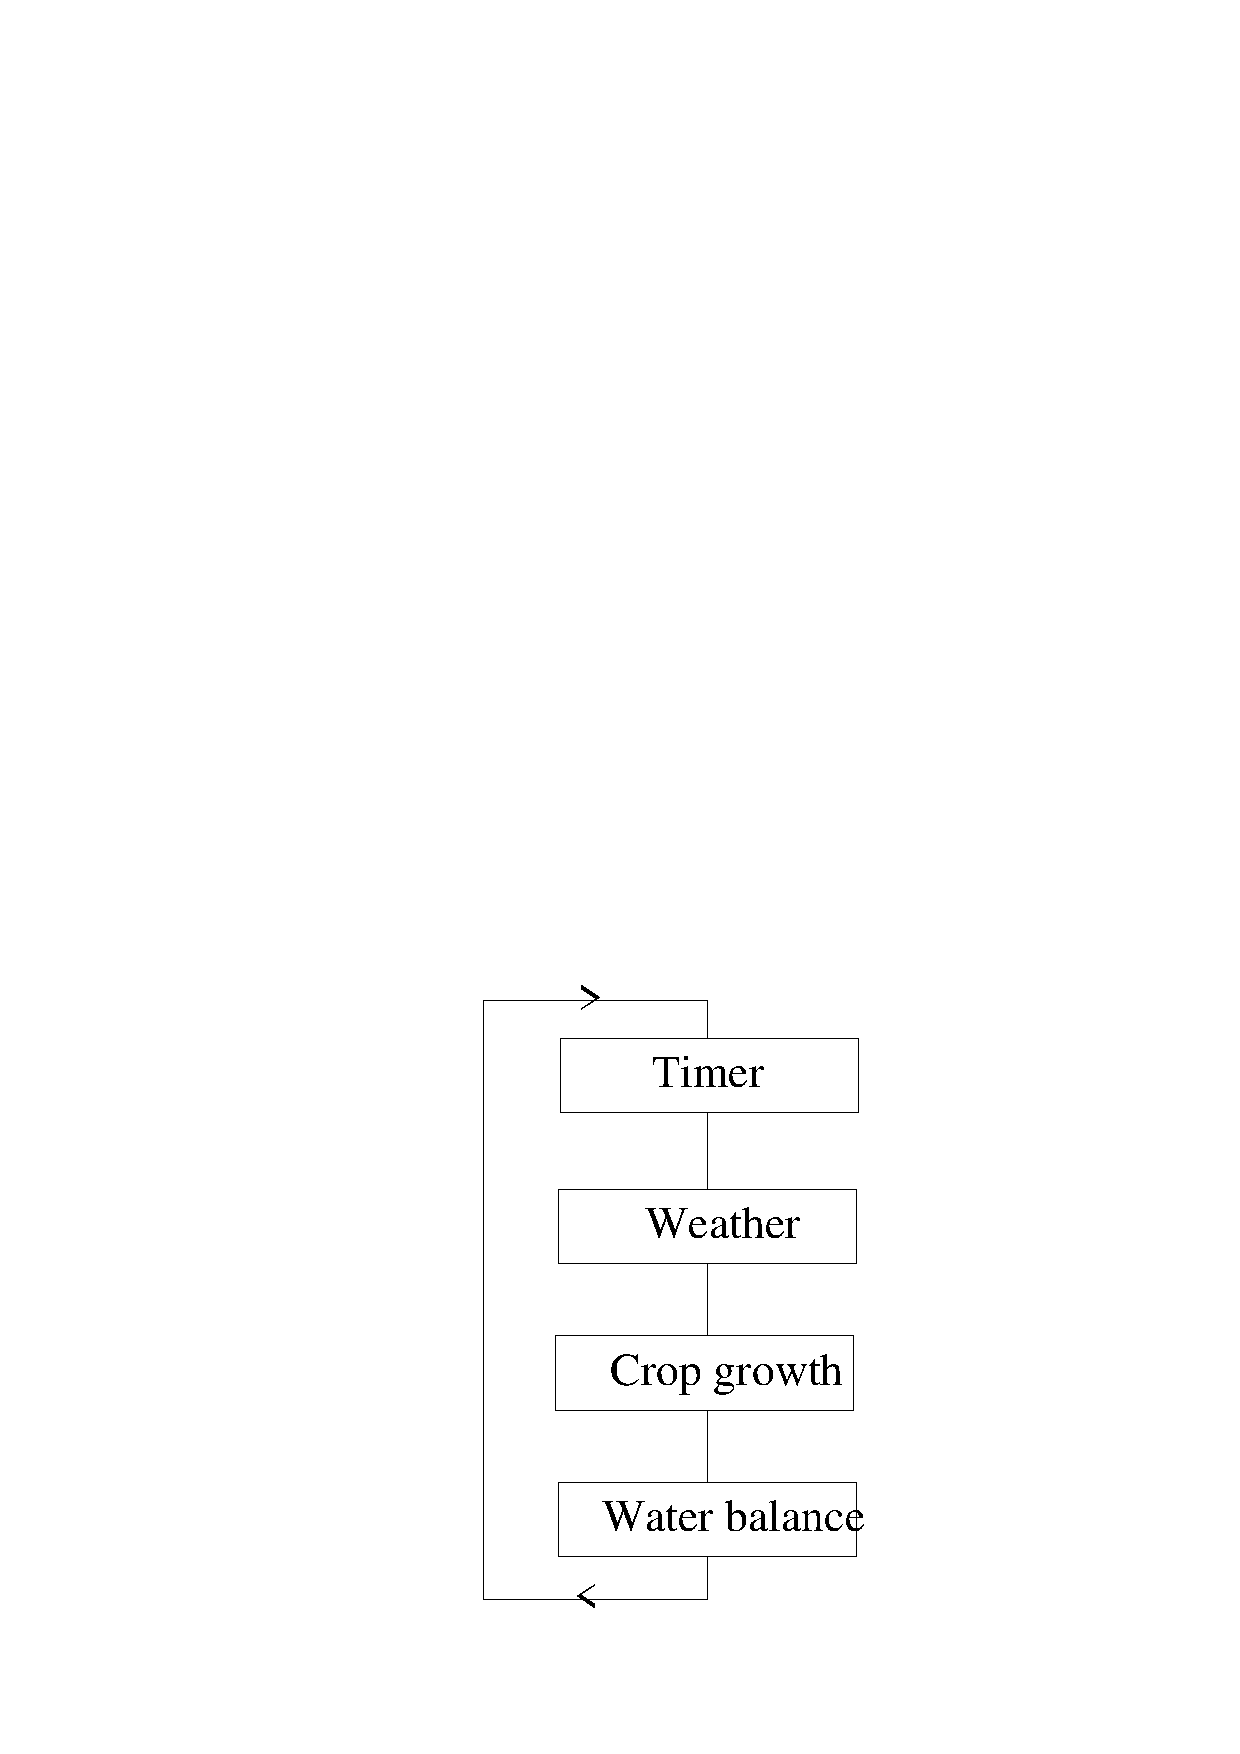
\includegraphics[width=80mm]{\FigDir/DAGLOOP.pdf}
\caption{Daily calculations of the simulation of crop growth}
% \begin{center}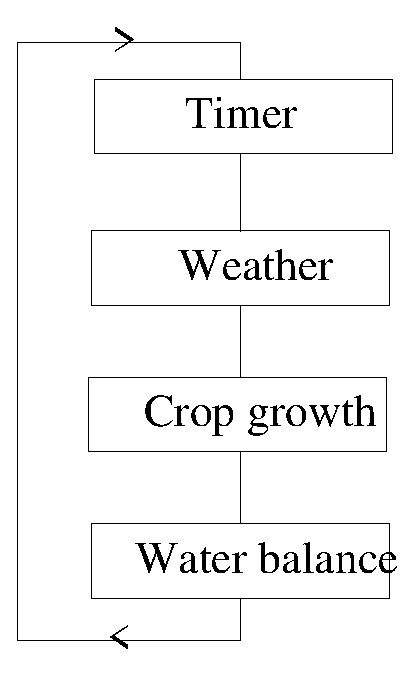
\epsfig{file=\FigDir/DAGLOOP.eps,width=8.04cm} \end{center}
\end{figure}

{\bf {\it Timer}}\\
In the WOFOST model, the Euler integration method is used to integrate the plant growth
processes over the growing period (i.e. all the time step executed). Therefore, the model
has to update the time and the time related variables each time the daily calcula\-tions are
performed. The subroutine TIMER takes care of this process, it controls the Euler
integration. The Euler integration method itself, is explained in chapter three.

{\bf {\it Weather}}\\
The meteorological parameters which are used by the WOFOST model are: maxi\-mum
temperature, minimum temperature, global radiation, windspeed, vapor pressure,
evapotranspiration and rainfall. In the WOFOST model, the Penman method is used to
calculate the evapotr\-anspiration. The weather related calculations of the model are
explained in chapter four.

Concerning the parameters global radiation and rainfall, it should be mentioned that in the
future JRC versions of WOFOST extra options to calculate this variable will be intro\-duced. 
Presently, in both versions the global radiation will be estimated using the \AA ngs\-tr\"{o}m 
formula when no actual data are available. The \AA ngs\-tr\"{o}m formula uses the sunshine
duration as input. If this parame\-ter is not available, in the subsequent JRC versions, the
global radiation will be estimated using either the equation proposed by Supit (1994) or
the Hargre\-aves formula (1985). 

The method developed by Supit, uses cloud cover and
maximum and minimum as input and its accuracy of the estimates comes close to the
accuracy of the \AA ngs\-tr\"{o}m estimates. The Hargreaves formula uses maximum and
minimum temperature only, and the accuracy of the estimates is less then either the 
\AA ngs\-tr\"{o}m formula or the method proposed by Supit.
Presently, the empirical coefficients of the \AA ngs\-tr\"{o}m formula have to be provided by the
user in the general version. In the JRC version these coefficient can be calculated as a
function of the latitude of the meteorological station.

Actual rainfall data are used as input in both versions. In the general version however, it
is also possible to use generated rainfall. For more informa\-tion about the differences
between these versions, one should consult Appendix 5.

{\bf {\it Crop growth}}\\
Crop growth depends on the daily net assimilation, which on its turn depends on the
intercepted light. The intercepted light is determined by the level of incoming radiation
and the leaf area of the crop. From the absorbed radiation and the photosynthetic
characteristics of single leaves, the daily rate of potential gross photosynthesis can be
calculated. Reduction of the transpiration due to water or oxygen stress results in a
reduced production of assimilates. The assimilates are partitioned over the various plant
organs. Figure \ref{fig:CropGrowthProcesses} presents a diagram of the crop growth processes. 
Chapter five explains in detail these processes.

\begin{figure}[htbp]
%Fig. 2.2
\centering
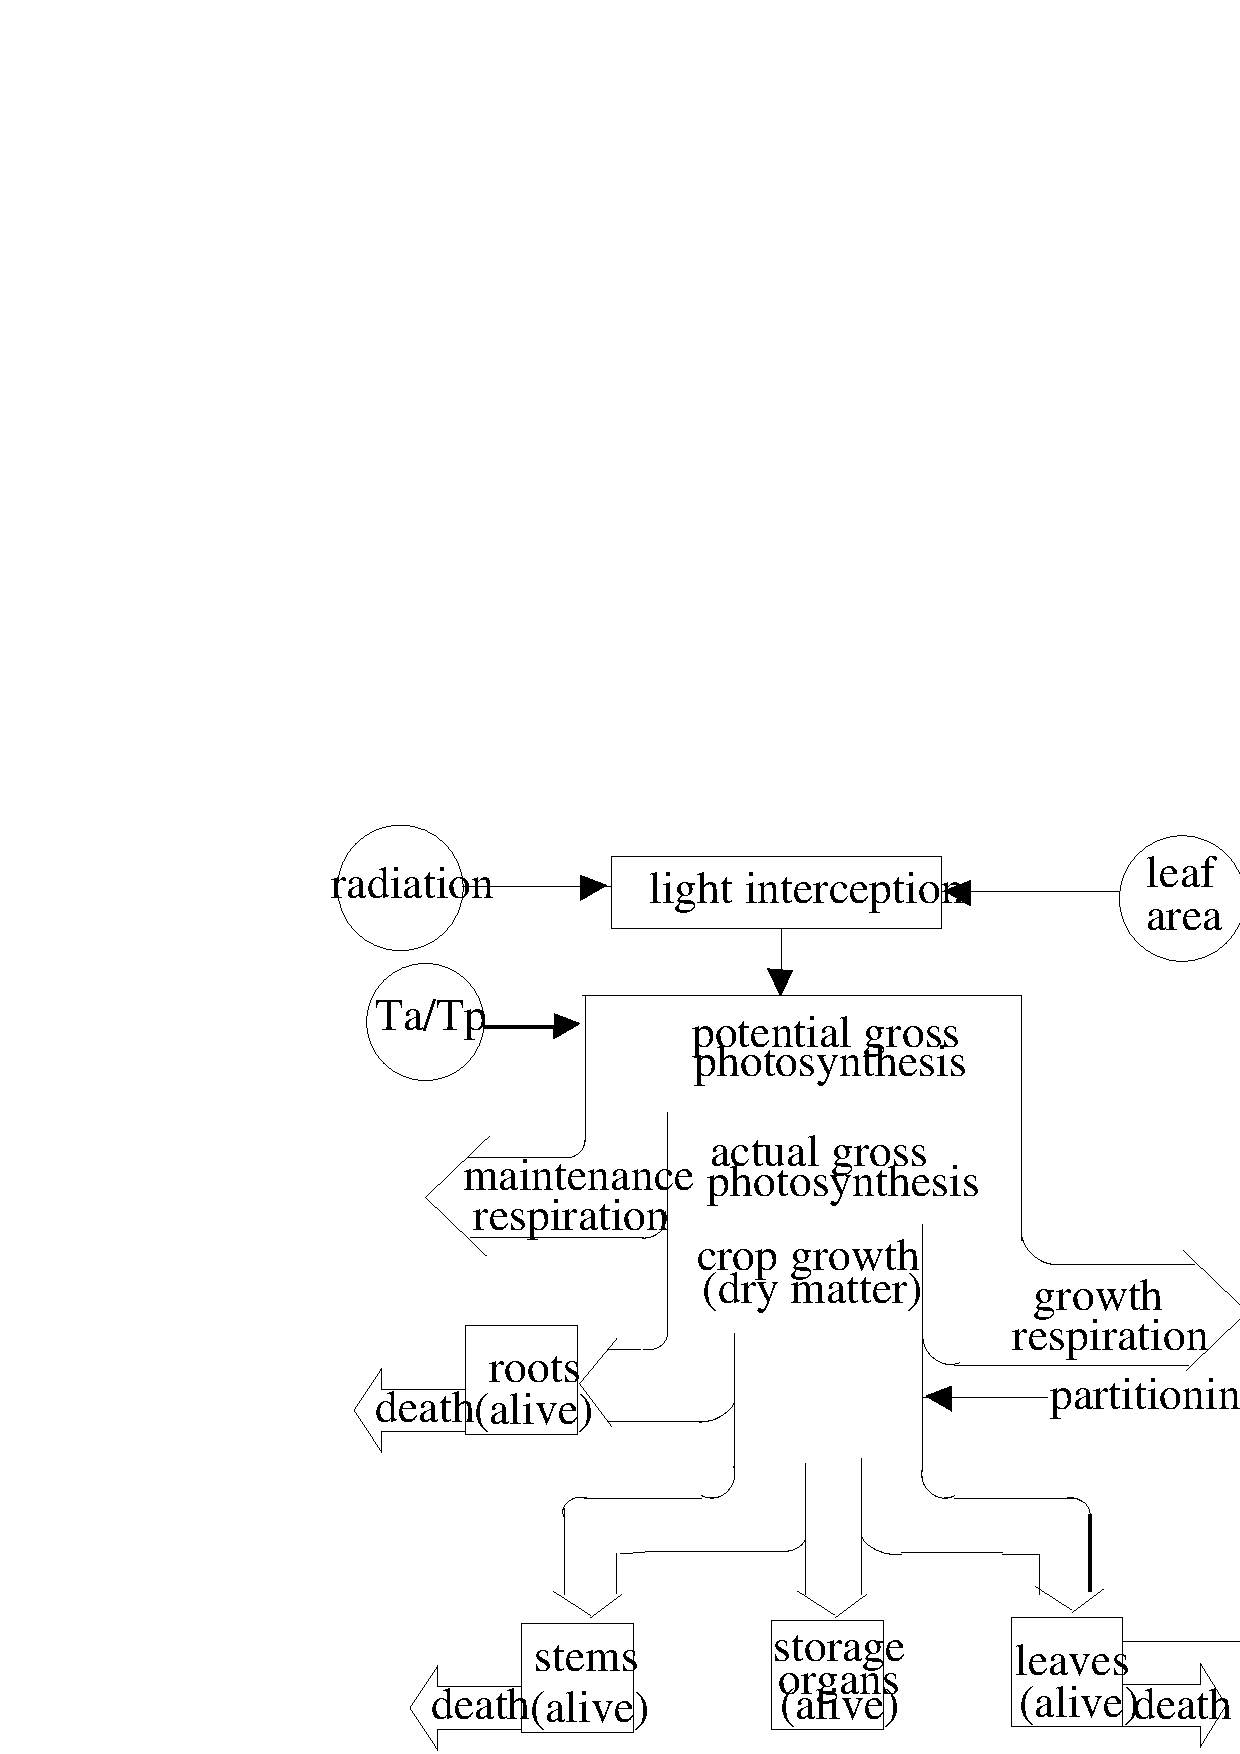
\includegraphics[width=\textwidth]{\FigDir/ASIMTREE.pdf}
\caption{Crop growth pro\-cesses. {\small T$_{{\rm a}}$ and T$_{{\rm p}}$ are actual and 
potential transpiration rate.} (de Koning, 1993)}
\label{fig:CropGrowthProcesses}
% \begin{center}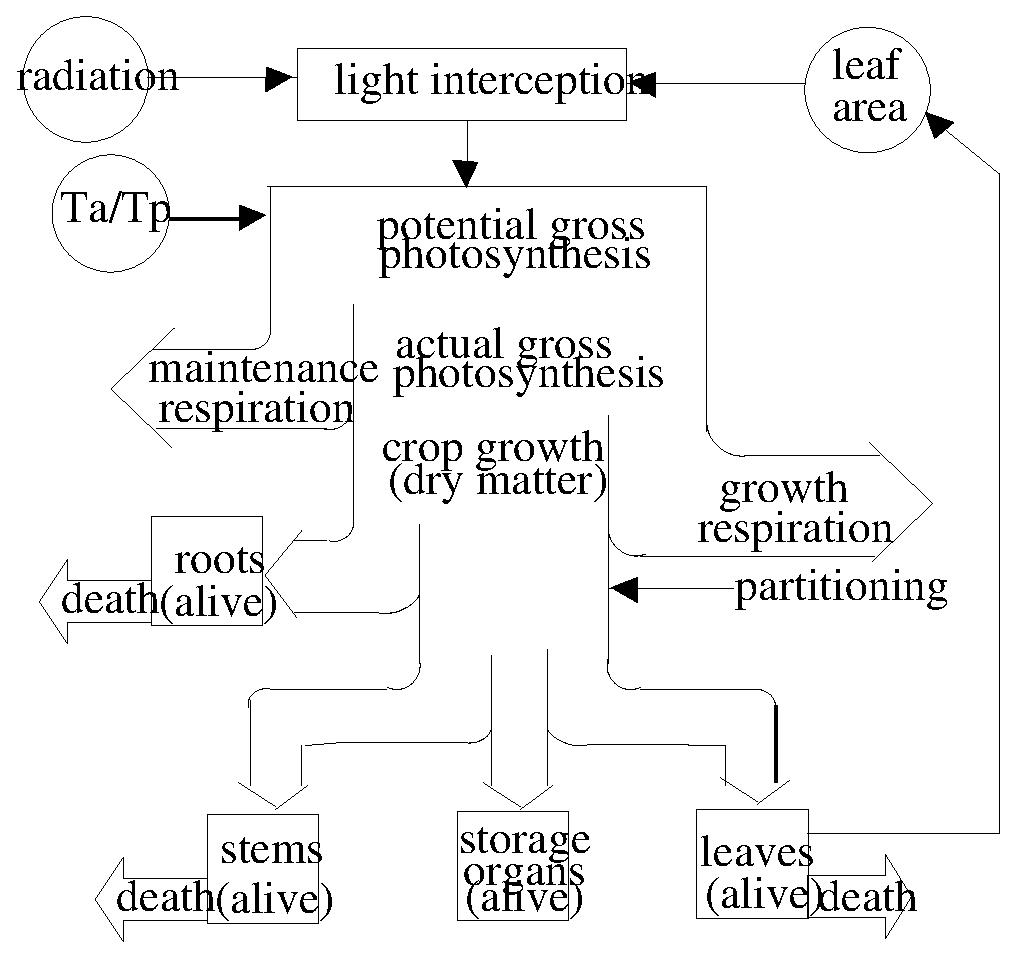
\epsfig{file=\FigDir/ASIMTREE.eps,width=\textwidth} \end{center}
\end{figure}

{\bf {\it Water balance}}\\
A crop growth simulation model also has to keep track of the soil moisture content to
deter\-mine when and to what degree a crop is exposed to water stress. This can be done
with the aid of a water balance, which com\-pares for a given period of time, incoming
water in the rooted surface soil with outgoing water and quantifies the difference between
the two as a change in the amount of soil moisture stored. The WOFOST model distin\-guishes 
three different situations. The first situation occurs when the soil moisture is at
field capacity and the crop growth reaches its potential level. In the second situation, the
influence of evapo(transpi)rati\-on and percolation on the availability of soil moisture are
considered. Production is dimin\-ished by the reduced availability of soil moisture. In the
last situation not only evapo(transpi)ration and percola\-tion are regarded but also influence
of groundwater is taken into account. Figure \ref{fig:waterbalances} illustrates the 
three possible situations in
the WOFOST model. Detailed information on this subject can be found in chapter six.

\begin{figure}[htbp]
%Fig. 2.3
\centering
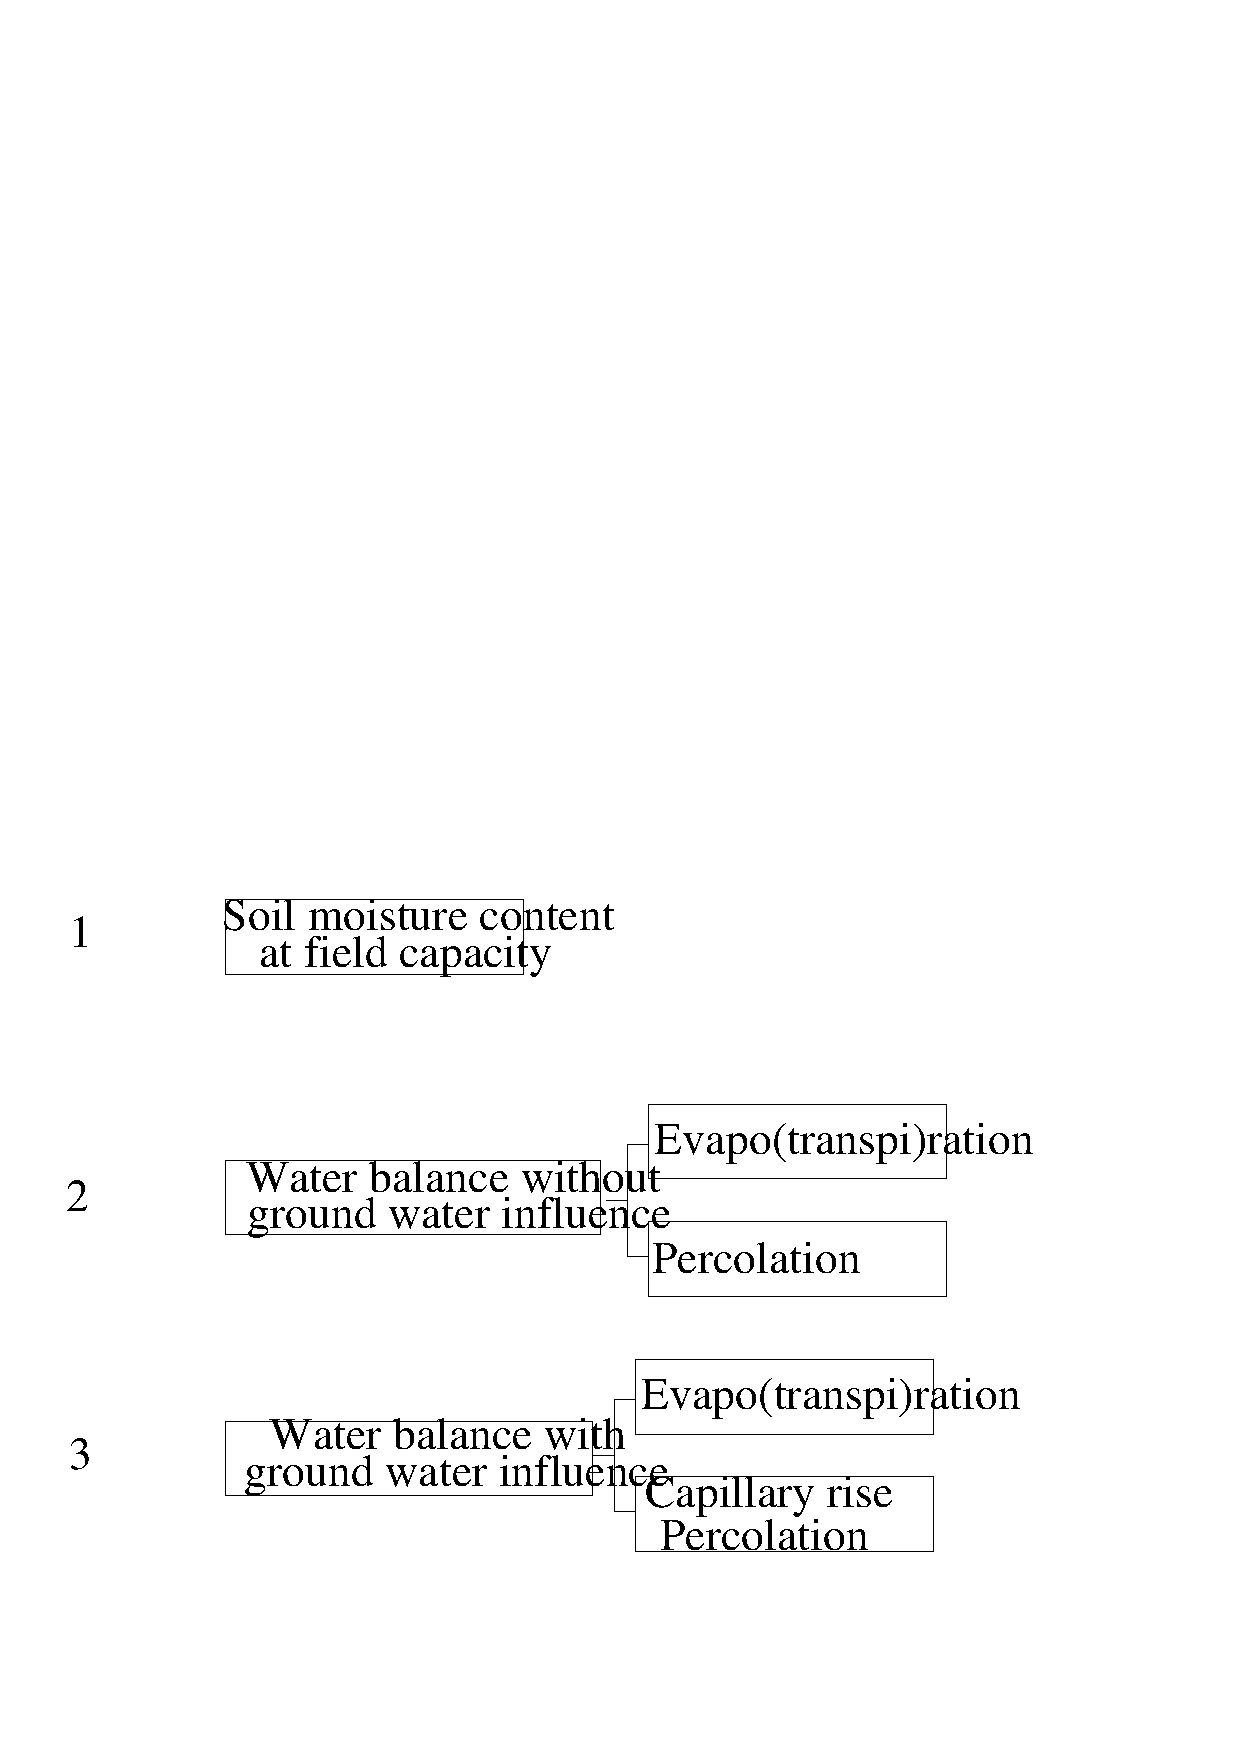
\includegraphics[width=140mm]{\FigDir/SOILLOOP.pdf}
\caption{The three possible situations of the water balance which are distin\-guished
by WOFOST 6.0.}
\label{fig:waterbalances}
% \begin{center}\epsfig{file=\FigDir/SOILLOOP.eps,width=\textwidth} \end{center}
\end{figure}

As mentioned before, the calculations of crop growth simulation are made on a daily
basis, (loop over days). WOFOST does also simulate crop growth for a number of growth
seasons. Only one growth season can be simulated for one cal\-endar year. Figure \ref{fig:YearlyCalc}
depicts the flow scheme of the yearly calculations (loop over years). The influ\-ence of
nutrients (nitrogen, phos\-phate and potassi\-um) on the yield and the yield statistics are
calculated on a yearly basis.

The procedure which calculates the nutrient requirements is based on the work of Janssen
et al (1990). The routine consist of four successive steps. First the potential supplies of
nitrogen, phosphorus and potassium are calculated, applying relationships between
chemical properties of the soil layer 0-20 cm and the maximum quantity of those nutrients
that can be absorbed by maize. It is assumed that the yield is not limited by nutrients and
growth factors. In the second step, the actual uptake of each nutrient is calculated as a
function of the potential supply of that nutrient, taking into account the potential supply of
the other two nutrients. The third step compromises the establishment of three yield
ranges as depending on the actual uptakes of nitrogen, phosphorus and potassium,
respectively. In step four these yield ranges are combined in pairs, and the yields
estimated for pairs of nutrients are averaged to obtain an ultimate yield estimate.

In the general WOF\-OST version, statis\-tics and the nutrient limited production are
included. In the JRC version of WOFOST 6.0 however, these features are omitted. See
Appendix 5.

\begin{figure}[htbp]
%Fig. 2.4
\centering
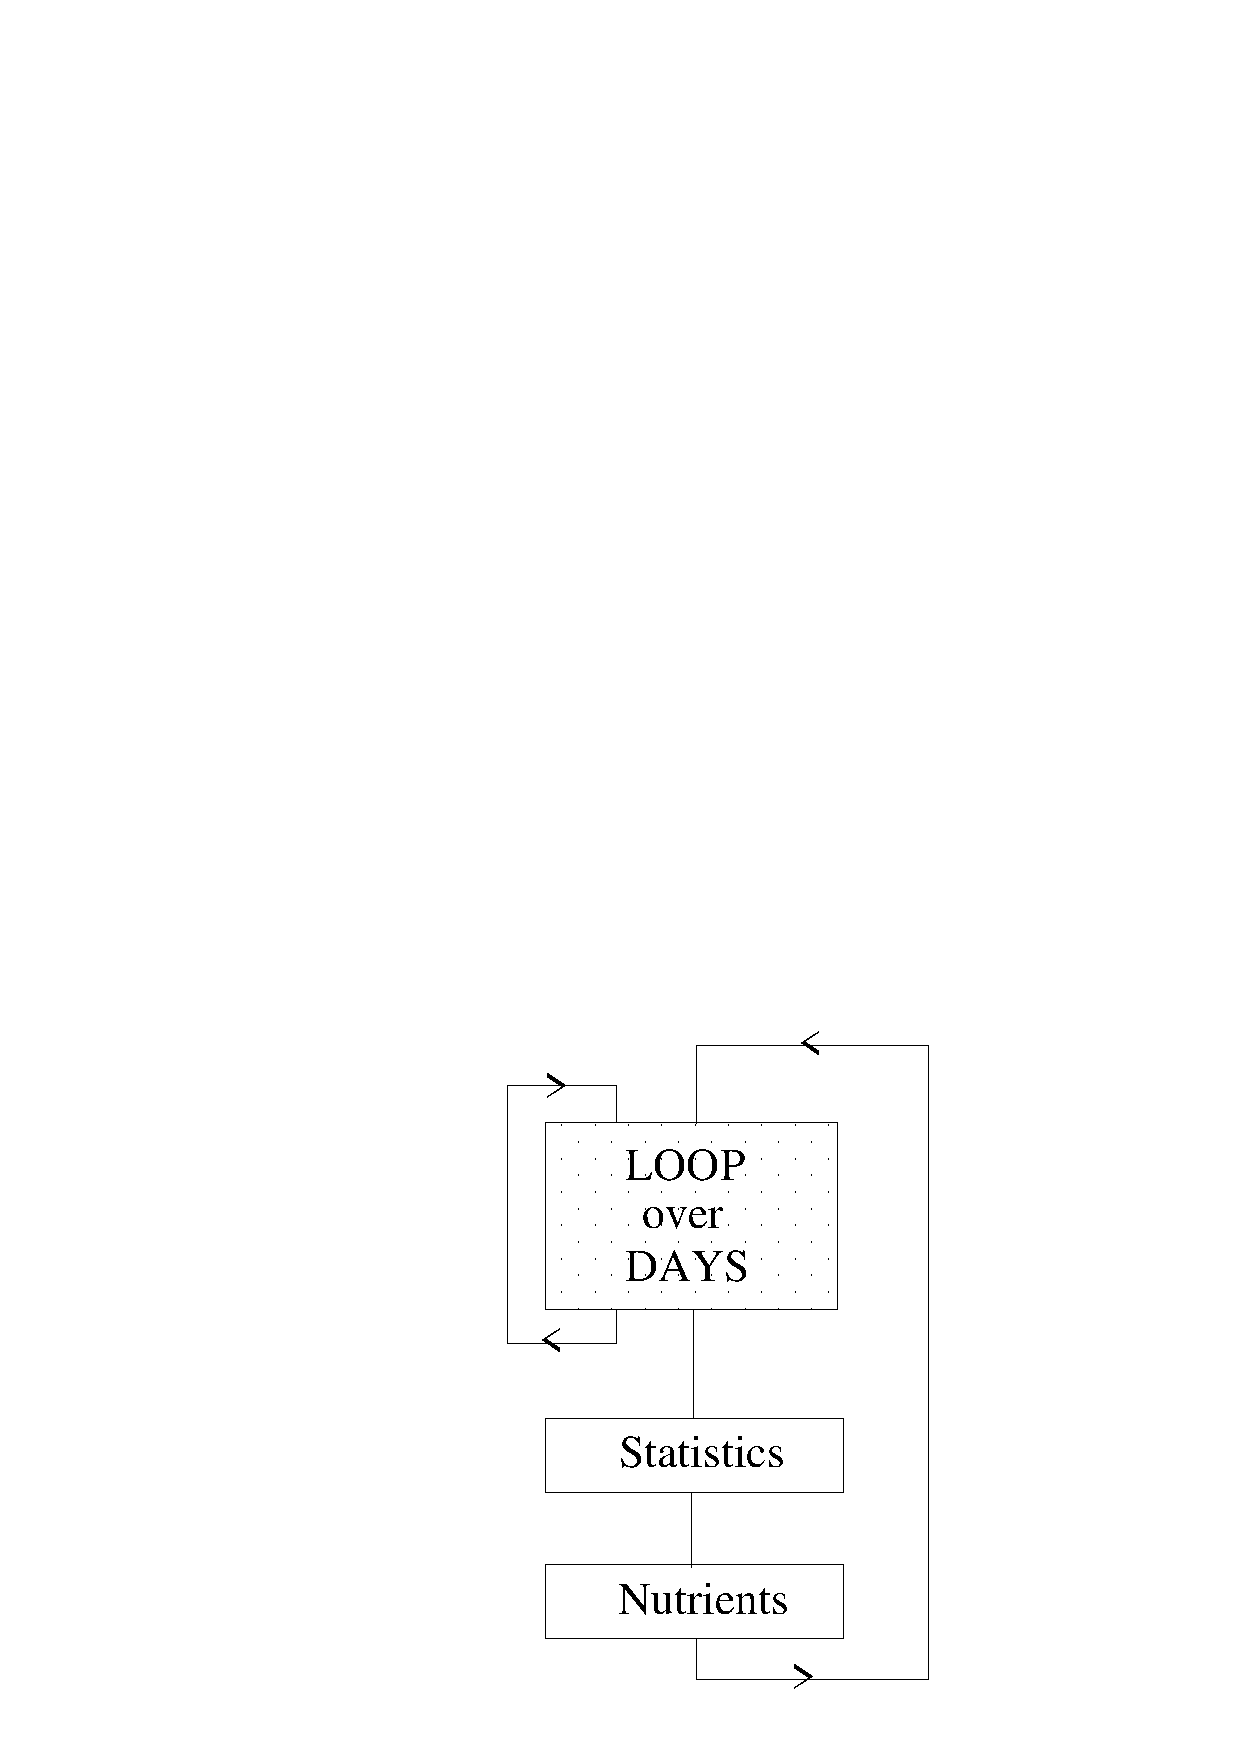
\includegraphics[width=80mm]{\FigDir/JAARLOOP.pdf}
\caption{Yearly calculations of the WOFOST model}
\label{fig:YearlyCalc}
% \begin{center}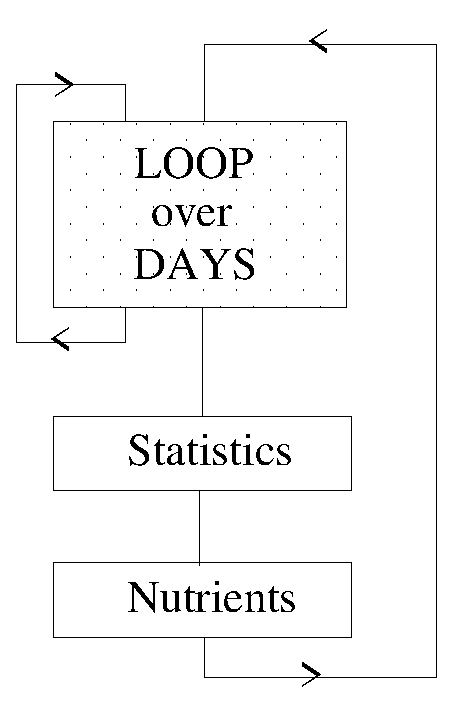
\epsfig{file=\FigDir/JAARLOOP.eps,width=8.04cm} \end{center}
\end{figure}
